\documentclass[english, fontsize=12pt, paper=a4, twoside=false, draft=true, pagesize=auto, version=last, DIV=16]{scrartcl}


\let\counterwithout\relax
\let\counterwithin\relax

\usepackage[utf8]{inputenc}
%Für Tabellen
\usepackage{tabularx}

% Für Absätze in Bildbeschreibung
\usepackage{caption}

% Zur nummerierten Aufzählung, mit automatischem Einrücken
\usepackage{paralist}
\usepackage{enumitem}
\usepackage{csquotes}


% mitwachsender Implikationspfeil mit Text
\makeatletter
\newcommand{\xRightarrow}[2][]{\ext@arrow 0359\Rightarrowfill@{#1}{#2}}
\makeatother


% Java Code Einbinden
\usepackage{listings}
\usepackage{color}
\usepackage[svgnames]{xcolor}



% Um einzelne Seiten zu drehen
\usepackage{pdflscape}
%\usepackage{rotating}
%\usepackage{lscape}


\usepackage{lmodern}
\usepackage[T1]{fontenc}
%\usepackage[latin1]{inputenc}
\usepackage{babel}
\usepackage[utf8]{inputenc}
\usepackage{stmaryrd}
\usepackage{extarrows}
\usepackage{ulem}



%Zur Bildnummerierung
\usepackage{chngcntr}
\usepackage{mathtools}
\usepackage{amsmath}
%Zur Verwendung von "chngcntr": \counterwithin{figure}{section}


%Euro-Zeichen
\usepackage{eurosym}

\usepackage{float}

\usepackage{amsmath}
\usepackage{acronym} %[''Optionen'']
\usepackage{esvect}  %Für Vektorpfeile, Aufruf mit \vv{Vektorname}

% Für schön Buchstaben1
\usepackage{mathrsfs}
\usepackage{suetterl}
\usepackage{calligra}

% Einzelne Seite drehen
\usepackage{lscape}


% ----------------------------------------------------------------------------------------
% ----------------------------------- Beginn Code einbinden ------------------------------
% ----------------------------------------------------------------------------------------
% Default fixed font does not support bold face
\DeclareFixedFont{\ttb}{T1}{txtt}{bx}{n}{12} % for bold
\DeclareFixedFont{\ttm}{T1}{txtt}{m}{n}{12}  % for normal

% Custom colors
\usepackage{color}
\definecolor{deepblue}{rgb}{0,0,0.5}
\definecolor{deepred}{rgb}{0.6,0,0}
\definecolor{deepgreen}{rgb}{0,0.5,0}

\usepackage{listings}

% Python style for highlighting
\newcommand\pythonstyle{\lstset{
language=Python,
basicstyle=\fontsize{10}{10}\selectfont\ttfamily,  % oder \ttm,
otherkeywords={self},             % Add keywords here
keywordstyle=\ttb\color{deepblue},
emph={MyClass,__init__},          % Custom highlighting
emphstyle=\ttb\color{deepred},    % Custom highlighting style
stringstyle=\color{deepgreen},
frame=tb,                         % Any extra options here
showstringspaces=false            %
}}


% Python environment
\lstnewenvironment{python}[1][]
{
\pythonstyle
\lstset{#1}
}
{}

% Python for external files
\newcommand\pythonexternal[2][]{{
\pythonstyle
\lstinputlisting[#1]{#2}}}


% ----------------------------------------------------------------------------------------
% ------------------------------------ Ende Code einbinden -------------------------------
% ----------------------------------------------------------------------------------------



%%% Neue Kommandos/Begriffe %%%
%\renewcommand{\thesection}{\arabic{section}}
% Für Fußnoten ohne Nummer
%\renewcommand{\thefootnote}{}



% Für die Normalschrift im Abkürzungsverzeichnis, das Paket "acronym" veranlasst eine andere Schriftart bei Abkürzungen.
\newcommand{\Rule}{\rule{\textwidth}{0.5mm}}
% \newcommand{\absatzParagraph}[1]{\paragraph{#1}\mbox{}\\}


\usepackage{geometry}
\newgeometry{left=18mm,right=18mm,top=15mm,bottom=15mm}
\footskip = 22pt

\usepackage{setspace}  % Paket einbinden
\onehalfspacing        % einstellen des Zeilenabstandes auf 1,5
\setlength{\parindent}{0in}
\usepackage{amsmath}
\usepackage[amsmath,amsthm,thmmarks]{ntheorem}
\usepackage{amssymb}


% Komplexitätsklassen
% \usepackage[bold,full]{complexity}


% Für Pseudocode
\usepackage{algorithm}
\usepackage{algpseudocode}


% für mehrzeilige Kommentare
\usepackage{verbatim}


% ------------- Beginn Definition von: Satz, Lemma Definition usw. -------------
\theoremstyle{break}
%\theoremstyle{definition}
\theorembodyfont{\upshape}
\newtheorem{defin}{Definition}[section] % Präambel
\newtheorem{lemma}[defin]{Lemma}
\newtheorem{satz}[defin]{Satz}
\newtheorem{kor}[defin]{Korollar}
\newtheorem{beo}[defin]{Beobachtung}
\newtheorem{bemerk}[defin]{Bemerkung}
\newtheorem{übung}[defin]{Übung}

%  ------------- Ende Definition von: Satz, Lemma Definition usw. -------------

% Für URLs
\usepackage{url}
\usepackage{hyperref}
\hypersetup{final}



\usepackage{animate}
\usepackage{graphicx}
\usepackage{graphics}
\usepackage{hyphenat}


\usepackage{tikz}
\usepackage{tkz-euclide}
\usetikzlibrary{arrows, matrix, shapes, decorations.pathmorphing,calc,patterns,through,intersections}

\newcommand*\bigO{\mathcal{O}}



\begin{document}


\title{
\vspace*{-10mm}
Exercise 5 \\[-3pt]
{\Large $\mathrm{for \ the \ lecture}$} \\[-3pt]
{\LARGE \textbf{Computational Geometry}}
}
\author{Dominik Bendle, Stefan Fritsch, Marcel Rogge and Matthias Tschöpe}
\maketitle
\vspace*{-10mm}

\section*{\large Exercise 1 (Nearest Neighbor Search in a Quadtree){\normalsize \hfill (4 points)}}

Data structures:

\begin{python}
class quadTree:
    def __init__(self, bound=None, ne=None, se=None, sw=None, nw=None):
        self.bound = bound # also include bounding box
        self.ne = ne
        self.se = se
        self.sw = sw
        self.nw = nw

class leaf:
    def __init__(self, val=None, bound=None):
        self.val = val
        self.bound = bound
\end{python}

Building the quadtree from a list:

\begin{python}
def createQuadTree(X, B=None):
    # g_MaxPts is a global variable
    if len(X) <= g_MaxPts:
        return leaf(X,B)

    # we will usually not do this here
    if not B:
        B = ( (min([x[0] for x in X]), max(x[0] for x in X))
            , (min([x[1] for x in X]), max(x[1] for x in X))
            )

    xsplit = (B[0][0]+B[0][1])/2
    ysplit = (B[1][0]+B[1][1])/2

    ne = []
    se = []
    sw = []
    nw = []

    for x in X:
        ise = x[0] >= xsplit
        isn = x[1] >= ysplit
        if isn and ise:
            ne.append(x)
        if isn and not ise:
            nw.append(x)
        if not isn and ise:
            se.append(x)
        if not isn and not ise:
            sw.append(x)

    # descend into the four subregions
    tNE = createQuadTree(ne, ((xsplit, B[0][1]), (ysplit, B[1][1])))
    tSE = createQuadTree(se, ((xsplit, B[0][1]), (B[1][0], ysplit)))
    tSW = createQuadTree(sw, ((B[0][0], xsplit), (B[1][0], ysplit)))
    tNW = createQuadTree(nw, ((B[0][0], xsplit), (ysplit, B[1][1])))
    return quadTree(bound=B, ne=tNE, se=tSE, sw=tSW, nw=tNW)
\end{python}

Finally, finding the nearest neighbor of a given point $x$ in the tree $T$:

\begin{python}
def findNearest(x, T, dist=np.inf, best=None):
    # check if dist radius intersects current region
    # if any of the inequalities hold, then there is nothing to do
    B = T.bound
    if x[0]+dist < B[0][0] \
            or x[0]-dist > B[0][1] \
            or x[1]+dist < B[1][0] \
            or x[1]-dist > B[1][1]:
                return (best, dist)

    if isinstance(T, quadTree):
        # search recursively in the children
        for t in [T.ne, T.se, T.sw, T.nw]:
            (best, dist) = findNearest(x, t, dist, best)

    if isinstance(T, leaf):
        for v in T.val:
            d = dist2d(x, v)
            if d < dist:
                best = v
                dist = d

    return (best, dist)
\end{python}

Sample command line output: A visualization is given in Figure~\ref{fig:q}, the black rectangles indicate all regions that are actually entered.

\begin{verbatim}
Time per Method:
naive:               5.108457999085658 ms
kd-tree:             0.12103399967600126 ms
quadtree:            0.2925829994637752 ms
Speedup (to naive):  17.459859282487596
Speedup (to kd):     0.4136740682056837
Both methods found same nearest point!
\end{verbatim}

\begin{figure}[tbhp]
  \centering
  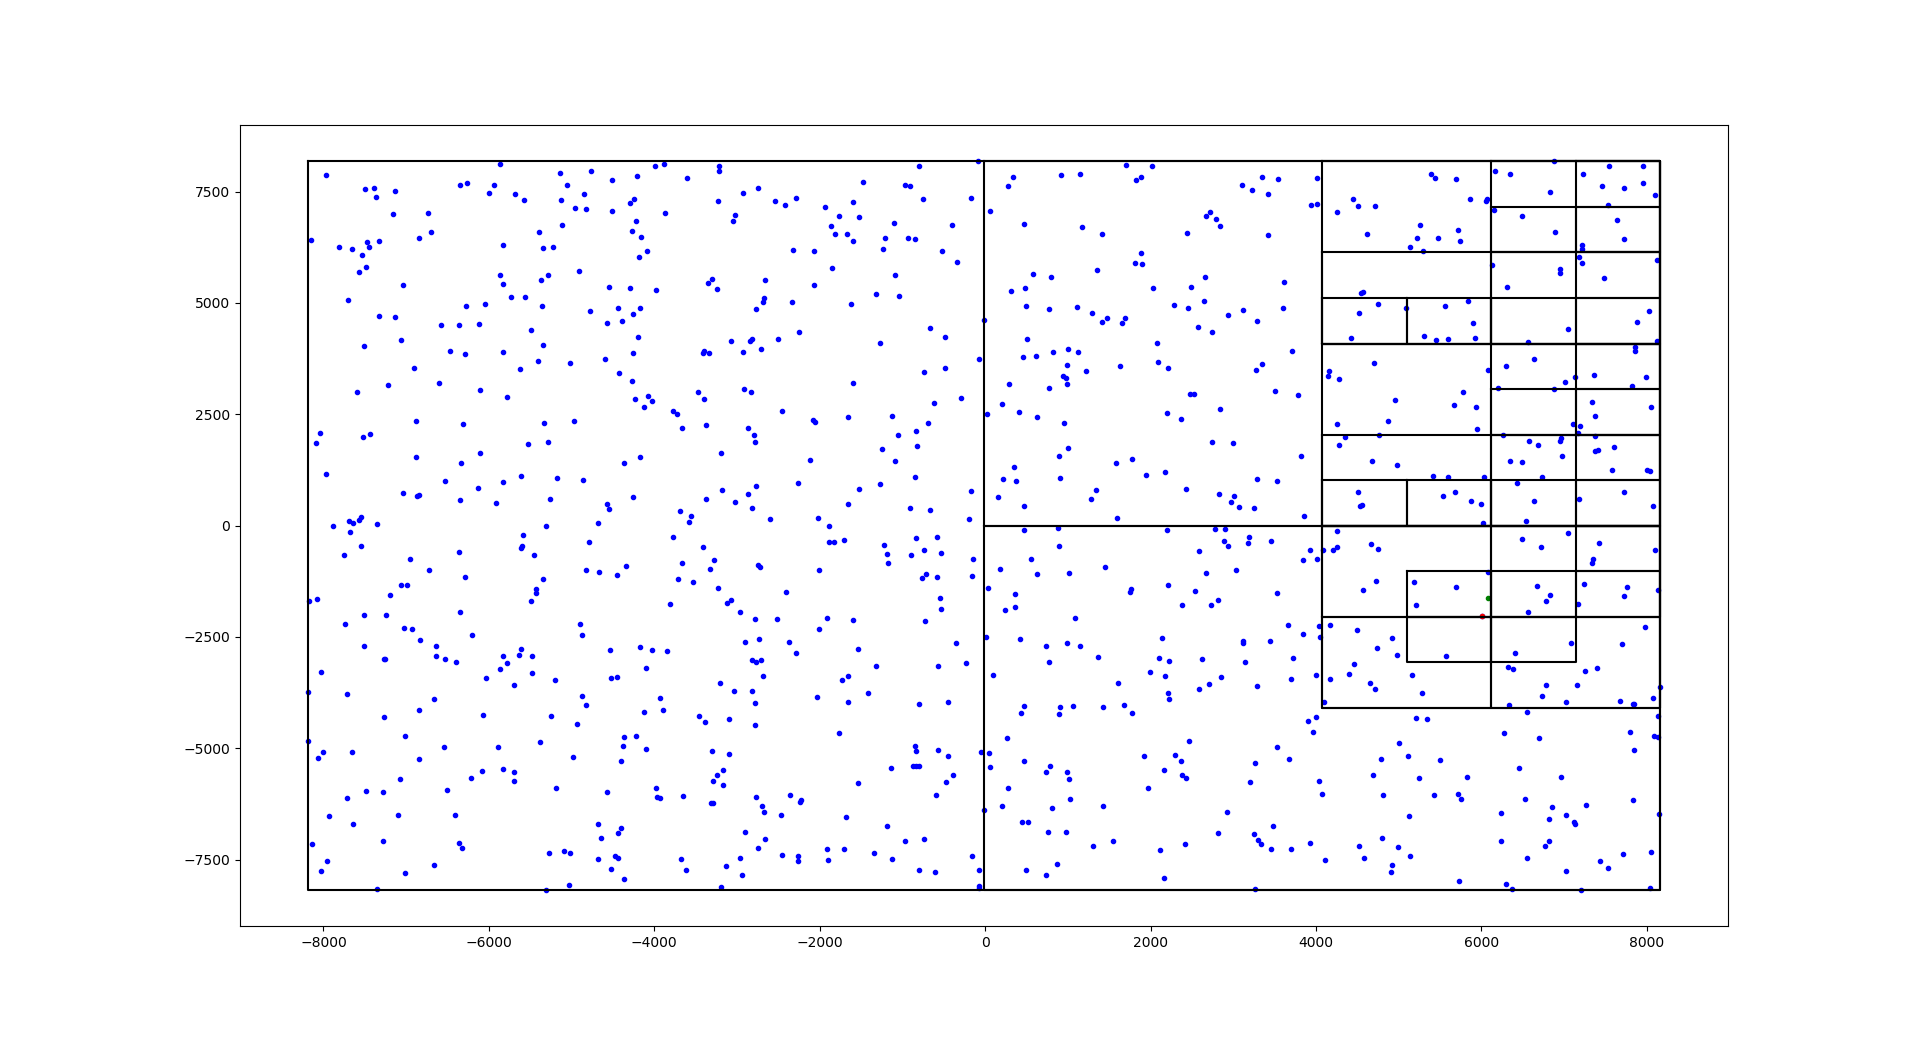
\includegraphics[width=0.99\textwidth]{./images/quadtrav.png}
  \caption{Nearest Neighbor Search}
  \label{fig:q}
\end{figure}

\newpage

\section*{\large Exercise 3 (Trapezoidal Map and Search Structure from a Planar Subdivision) {\normalsize \hfill (5 points)}}

\begin{center}
  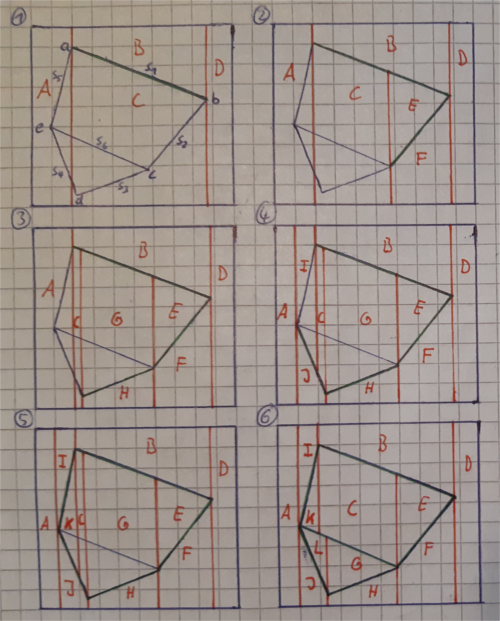
\includegraphics[width=0.99\textwidth]{./images/map.png}
\end{center}

\begin{center}
  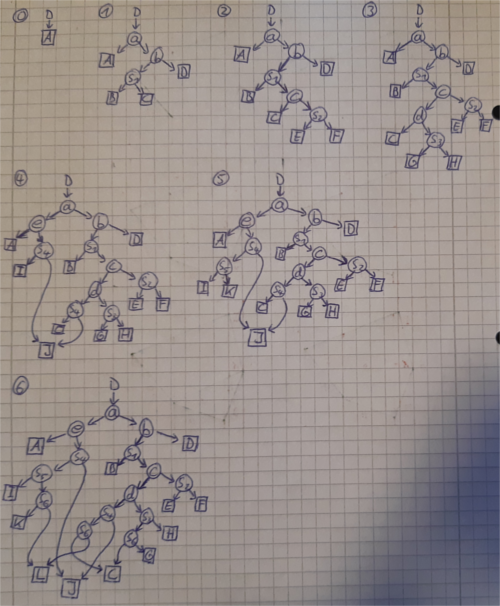
\includegraphics[width=0.99\textwidth]{./images/datastructure.png}
\end{center}


\end{document}

